\documentclass[11pt]{paper}
\usepackage{palatino}
\usepackage{amsfonts,amsmath,amssymb}
% \usepackage{graphicx}

\usepackage{listings}
\usepackage{textcomp}
\usepackage{color}

\definecolor{dkgreen}{rgb}{0,0.6,0}
\definecolor{gray}{rgb}{0.5,0.5,0.5}
\definecolor{mauve}{rgb}{0.58,0,0.82}

\lstset{frame=tb,
  language=R,
  aboveskip=3mm,
  belowskip=3mm,
  showstringspaces=false,
  columns=flexible,
  basicstyle={\small\ttfamily},
  numbers=none,
  numberstyle=\tiny\color{gray},
  keywordstyle=\color{blue},
  commentstyle=\color{dkgreen},
  stringstyle=\color{mauve},
  breaklines=true,
  breakatwhitespace=true,
  tabsize=3
}



\ifx\pdftexversion\undefined
    \usepackage[dvips]{graphicx}
\else
    \usepackage[pdftex]{graphicx}
    \usepackage{epstopdf}
    \epstopdfsetup{suffix=}
\fi

\usepackage{subfig}


% This allows pdflatex to print the curly quotes in the
% significance codes in the output of the GAM.
\UseRawInputEncoding

\begin{document}

%%%%%%%%%%%%%%%%%%%%%%%%%%%%%%%%%%%%%%%%
% Problem Set 7
%%%%%%%%%%%%%%%%%%%%%%%%%%%%%%%%%%%%%%%%

\pagestyle{empty}
{\noindent\bf Spring 2021 \hfill Ali Berra}
\vskip 16pt
\centerline{\bf University of Central Florida}
\centerline{\bf College of Business}
\vskip 16pt
\centerline{\bf QMB 6911}
\centerline{\bf Capstone Project in Business Analytics}
\vskip 10pt
\centerline{\bf Solutions:  Problem Set \#9}
\vskip 32pt
\noindent
% 
\section{Data Description}

This analysis follows the script \texttt{Trucks\_Reg\_Model.R} to produce a more accurate model for used trucks cost with the data from \texttt{UsedTrucks.dat} in the \texttt{Data} folder. 
The dataset includes the following variables.
\begin{table}[h!]
\begin{tabular}{l l l}

$type_i$ & = & sale type \\

$pauc$ & = & price when sold at auction \\
$ pret$ & = &price when sold retail \\ 
$mileage$ & = & odometer \\ %, $0$ otherwise \\
$make$ & = &make of vehicule \\
$year$ & = &model year of vehicle \\ 
$damage$ & = & an index of damage to vehicle, 1 little damage, 10 a lot\\
$dealer$ & = & dealer id \\ 
$ror$& = &rate-of-return\\
$cost$& = &net amount given to trade in\\


\end{tabular}
\end{table}
%
From problem set 7, we build a model that can predict the cost of the vehicule depending 
on the damage of the trucks. we will add quadratic specification for damage 
which will increase the relationship between cost and damage. 



%%%%%%%%%%%%%%%%%%%%%%%%%%%%%%%%%%%%%%%%
\clearpage
\section{Linear Regression Model}
%%%%%%%%%%%%%%%%%%%%%%%%%%%%%%%%%%%%%%%%

A natural staring point is the recommended linear model
from Problem Set \#7. 

\subsection{Quadratic Specification for Damage}

we can say that the more a Truck is damaged the less likely it will sell. 
to impliment this in the model we squared the damage variable to have more impact inthe realtionship.


The results of this regression specification are shown in 
Table \ref{tab:reg_sq_damage}. 
% 

\begin{table}
\begin{center}
\begin{tabular}{l c}
\hline
 & Model 1 \\
\hline
(Intercept)     & $8.76488^{***}$  \\
                & $(0.08135)$      \\
squared\_damage & $0.00459^{*}$    \\
                & $(0.00214)$      \\
make            & $-0.00619$       \\
                & $(0.00537)$      \\
damage          & $-0.04677$       \\
                & $(0.02543)$      \\
dealer          & $0.00196$        \\
                & $(0.00417)$      \\
mileage         & $-0.00001^{***}$ \\
                & $(0.00000)$      \\
age             & $-0.07163^{***}$ \\
                & $(0.01114)$      \\
type            & $0.04438^{*}$    \\
                & $(0.02182)$      \\
\hline
R$^2$           & $0.19087$        \\
Adj. R$^2$      & $0.19029$        \\
Num. obs.       & $9861$           \\
\hline
\multicolumn{2}{l}{\scriptsize{$^{***}p<0.001$; $^{**}p<0.01$; $^{*}p<0.05$}}
\end{tabular}
\caption{Quadratic Model for Trucks cost}
\label{tab:reg_sq_damage}
\end{center}
\end{table}

% 
according to our model milage and age are more significant predictor than damge with -5.053e-06 and -7.163e-02 coeffiecient respectively. 
the P value for damage 0.06 and for squared damage 0.03 which is slightly significant when squared







%%%%%%%%%%%%%%%%%%%%%%%%%%%%%%%%%%%%%%%%
\clearpage
\section{Nonlinear Specifications}
%%%%%%%%%%%%%%%%%%%%%%%%%%%%%%%%%%%%%%%%


% \clearpage
\subsection{Nonparametric Specification for Damage}


The specification in 
Table \ref{tab:reg_sq_damage}
assumes a quadratic functional form for
the relationship between cost and damage. 
To consider the damage variable alone, 
while accounting for the effects of other variables, 
one can fit a nonparametric model to the residuals 
from a model of Trucks cost, 
after regressing Trucks cost on the other variables. 
This leaves only the variation in trucks cost that is not explained by the other variables. 
Going one step further, perform the same transformation to the damage variable:
take the residuals from a model of damage, 
after regressing damage on the other variables. 
This allows a model that would fit exactly the same as if it were estimated within a full model with all variables included. 




\pagebreak 
To illustrate the fit of the model, 
Figure \ref{fig:dev_vs_cost} shows a scatter plot 
of the residual log cost on damage. 
The observations are shown in blue
and the fitted values are shown in red.
The variation in the fitted values results from the 
fact that it is not plotted against the transformed excess damage variable used in the regressions.
Still, the quadratic pattern is apparent
and appears to match the data. 

\begin{figure}[h!]
  \centering
  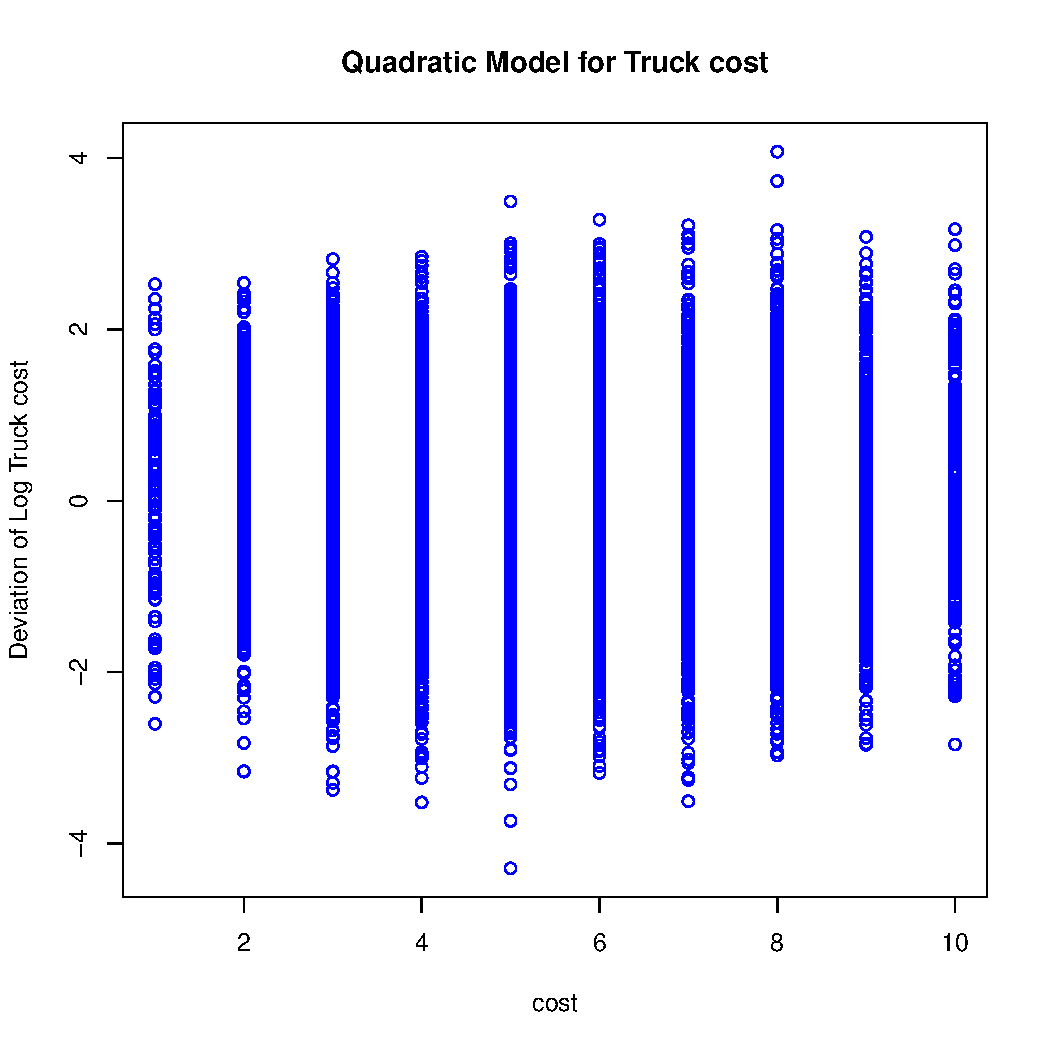
\includegraphics[scale = 0.5, keepaspectratio=true]{../Figures/dev_vs_cost}
  \caption{Linear-Quadratic Model for Truck cost} \label{fig:dev_vs_cost}
\end{figure}



\pagebreak
As a comparison, Figure \ref{fig:dev_vs_damage_dev} 
augments the above by showing the plot against the 
residuals from the regression for damage:
the ``excess damage'' compared to what would be 
expected given the other characteristics of a truck. 



\begin{figure}[h!]
  \centering
  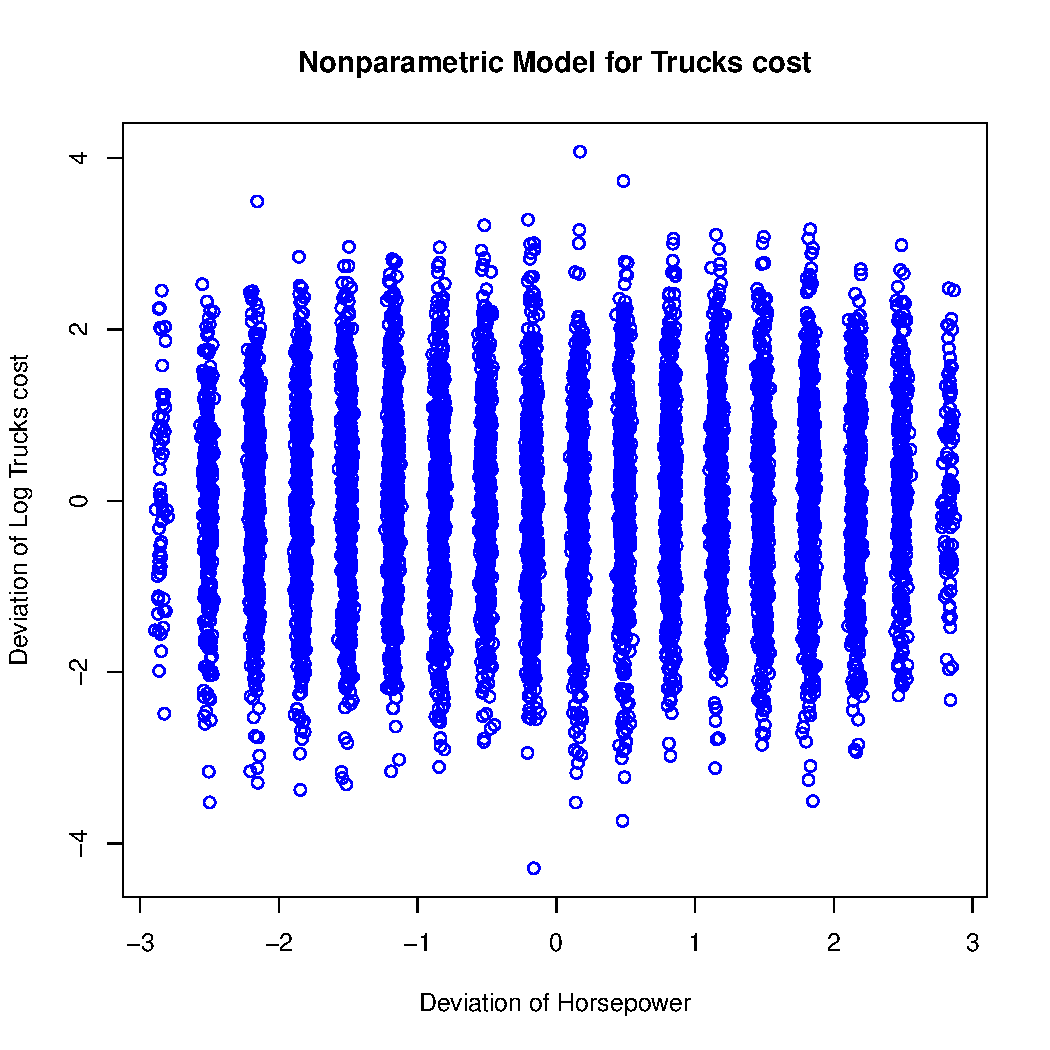
\includegraphics[scale = 0.5, keepaspectratio=true]{../Figures/dev_vs_cost_dev}
  \caption{Linear-Quadratic Model for Tractor Prices: damage} \label{fig:dev_vs_cost_dev}
\end{figure}

\clearpage
Now consider a nonparametric specification for 
the relationship between cost and damage.
Figure \ref{fig:dev_np_vs_damage_dev} 
overlays the nonparametric estimate (shown in green) with the above in 
Figure \ref{fig:dev_vs_damage_dev}.
The pattern has more variation in slope but 
closely follows the prediction from the quadratic model. 
So far, it appears that the quadratic form
is close enough.

\begin{figure}[h!]
  \centering
  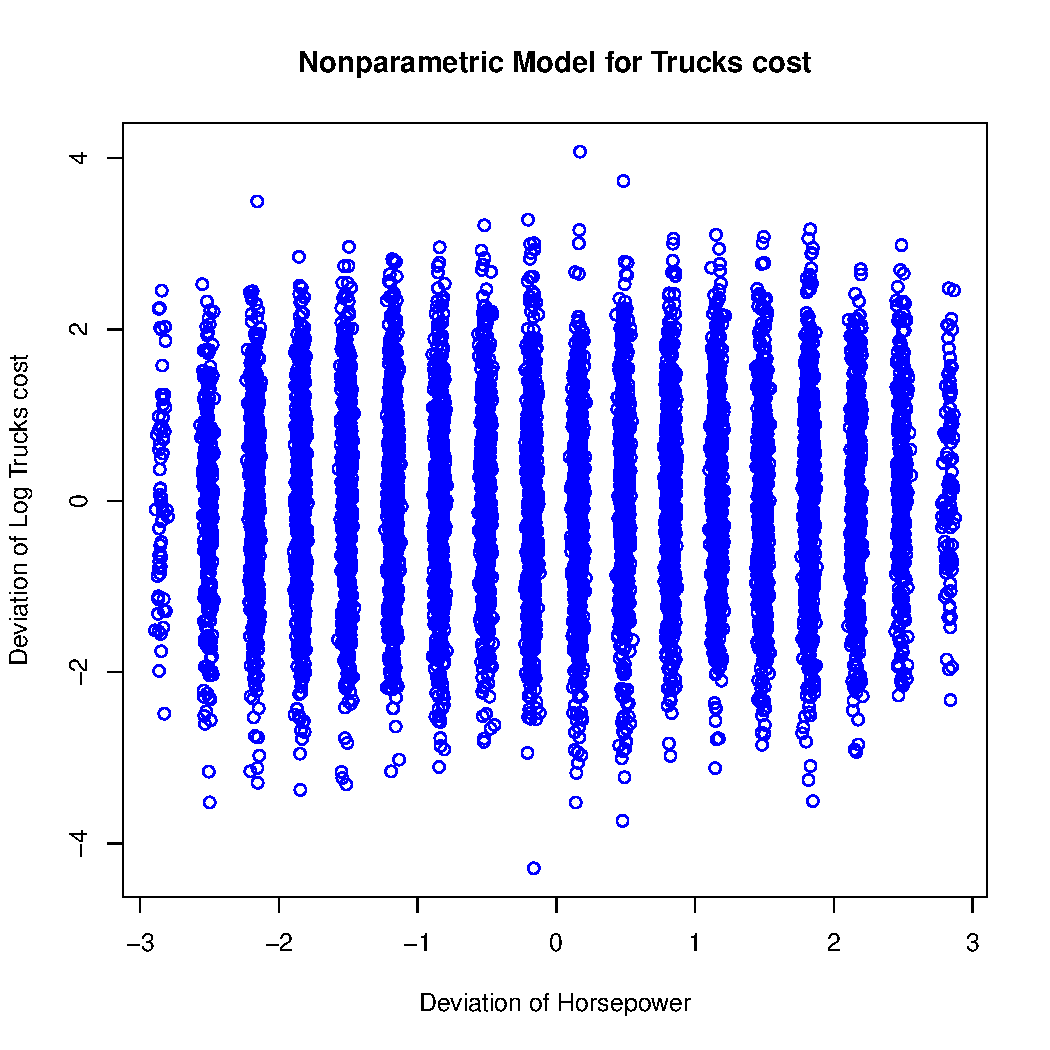
\includegraphics[scale = 0.5, keepaspectratio=true]{../Figures/dev_np_vs_damage_dev}
  \caption{Nonparametric Model for Tractor Prices: Damage} \label{fig:dev_np_vs_damage_dev}
\end{figure}

 
\clearpage



\subsection{Nonparametric Specification for Age}

As above, first conduct FWL regressions 
to reduce the problem to two dimensions. 
% 
To illustrate the fit of the model, 
Figure \ref{fig:dev_np_vs_age_dev} 
shows a scatter plot 
of the residual log cost on 
the residuals from the regression for age:
the ``excess age'' of a truck compared to what would be 
expected given the other characteristics of the Truck. 
% 
The observations are shown in blue
and the fitted values are shown in red.

Next we considered a nonparametric specification for 
the relationship between cost and age.
% 
Figure \ref{fig:dev_np_vs_age_dev} 
overlays the nonparametric estimate (shown in green) 
with the linear model.
The pattern has more variation in slope but 
closely follows the prediction from the linear model. 
Although the nonparametric estimate varies around the linear estimate,
it appears that the linear form
is a close enough approximation without the added complexity.
Next, I will revisit the remaining continuous variable.


\begin{figure}[h!]
  \centering
  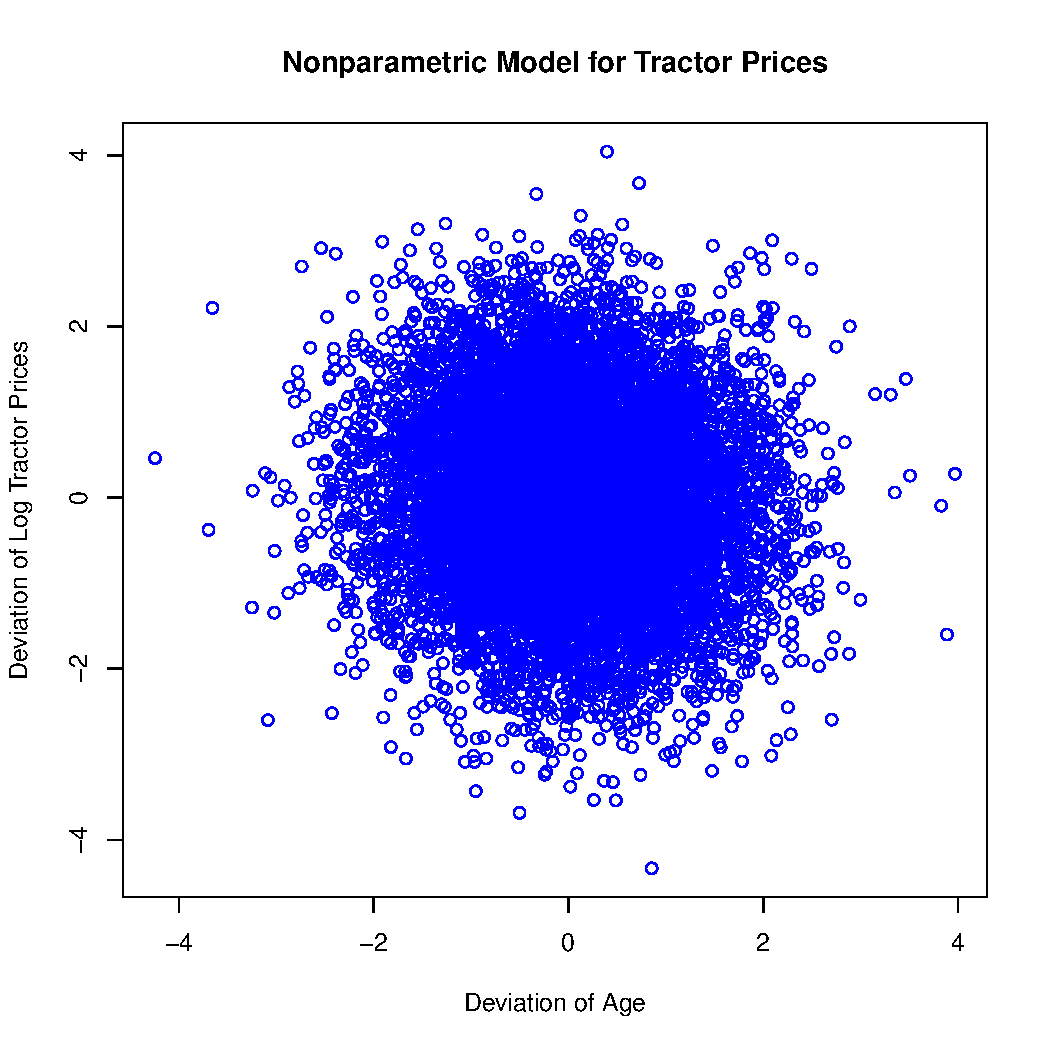
\includegraphics[scale = 0.5, keepaspectratio=true]{../Figures/dev_np_vs_age_dev}
  \caption{Nonparametric Model for Tractor Prices: Excess Age} \label{fig:dev_np_vs_age_dev}
\end{figure}



\clearpage
\subsection{Nonparametric Specification for mileage}

As above, first conduct FWL regressions 
to reduce the problem to two dimensions. 
%
To illustrate the fit of the model, 
Figure \ref{fig:dev_np_vs_eng_dev}
shows a scatter plot 
of the residual log cost on 
residuals from the regression for mileage:
the ``excess mileage'' of a Truck compared to what would be 
expected given the other characteristics of the Truck. 
The observations are shown in blue
and the fitted values are shown in red.
As with age, the linear fit follows a straight line,
since we have a single variable with no
quadratic transformation.
% 
I moved directly to the nonparametric specification for 
the relationship between prices and engine hours.
Figure \ref{fig:dev_np_vs_eng_dev} 
overlays the nonparametric estimate, shown in green. 
The pattern has more variation in slope but 
closely follows the prediction from the linear model. 
Although the nonparametric estimate varies around the linear estimate,
it appears that the linear form
is also a close enough approximation, 
just as was found for the age variable.


\begin{figure}[h!]
  \centering
  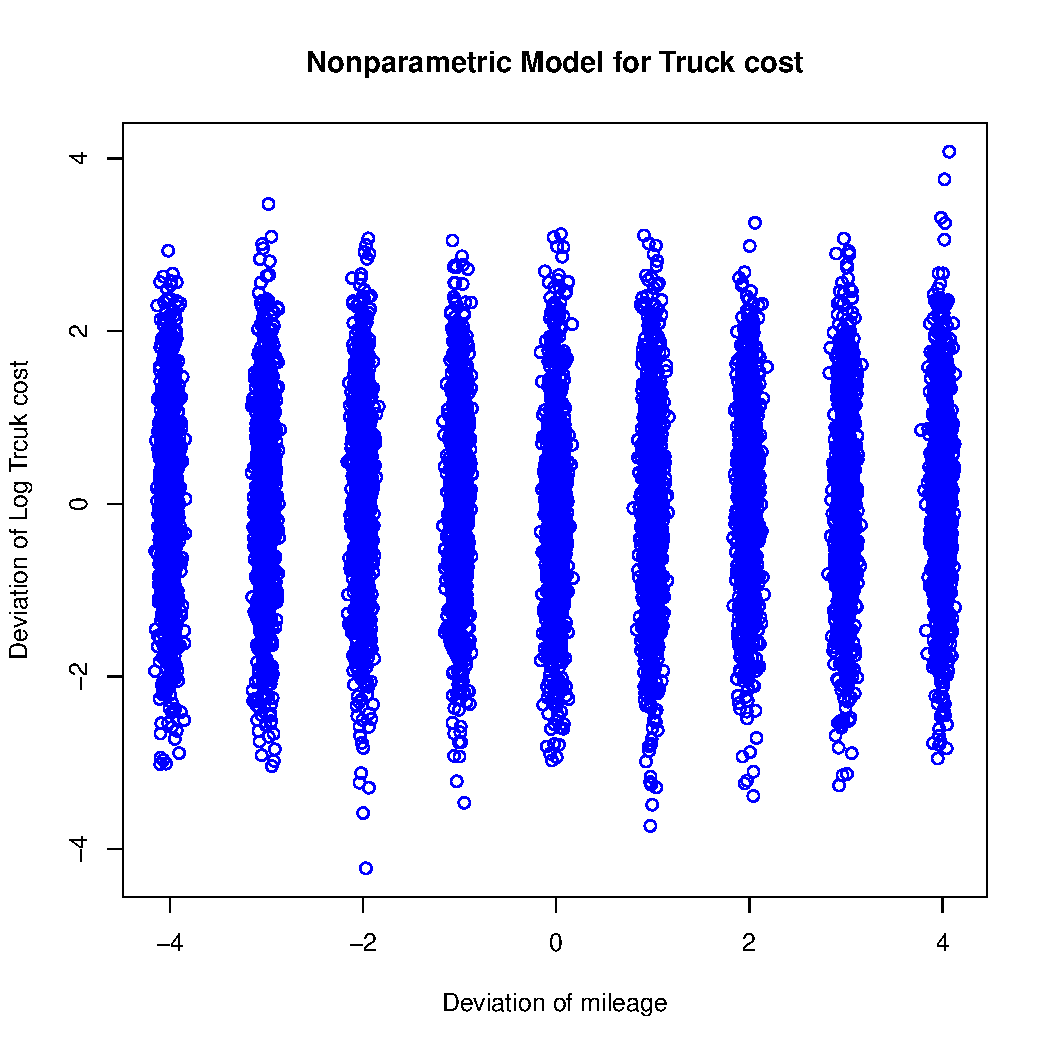
\includegraphics[scale = 0.5, keepaspectratio=true]{../Figures/dev_np_vs_eng_dev}
  \caption{Nonparametric Model for Tractor Prices: Excess Engine Hours} \label{fig:dev_np_vs_eng_dev}
\end{figure}
\pagebreak
\section{Semiparametric Estimates}

As I was building the above nonparametric models, 
I stored the predictions and will now use them as variables in 
linear models. 
Table \ref{tab:reg_semipar} 
shows the estimates from a set of models. 
Model 1 is the benchmark linear model in 
Table \ref{tab:reg_sq_horse}. 
Model 2 is a semi-parametric model
with a nonparametric fit on horsepower
substituted in for the horsepower variables.
Models 3 and 4 are semi-parametric models
with nonparametric fits on age and engine hours, respectively.
Model 5 is a maximally semiparametric model, 
with nonparametric fits for all continuous variables. 
For each of the single-variable semiparametric models, 
the coefficients are near one
and the fits are similar to the linear model. 
Even with maximal flexibility, the fit of Model 5
is not much better than the benchmark linear model. 
Across all models, the adjusted $\bar{R}^2$ values are all hovering around 0.80. 
All things considered, these are excellent models
and the linear model is sufficient.


\begin{table}
\begin{center}
\begin{tabular}{l c c c c c}
\hline
 & Model 1 & Model 2 & Model 3 & Model 4 & Model 5 \\
\hline
(Intercept)     & $8.76488^{***}$  & $8.65711^{***}$  & $8.95824^{***}$  & $8.76488^{***}$  & $8.74458^{***}$ \\
                & $(0.08135)$      & $(0.05515)$      & $(0.07530)$      & $(0.08135)$      & $(0.11028)$     \\
squared\_damage & $0.00459^{*}$    &                  & $0.00454^{*}$    & $0.00459^{*}$    &                 \\
                & $(0.00214)$      &                  & $(0.00213)$      & $(0.00214)$      &                 \\
make            & $-0.00619$       & $-0.00619$       & $-0.00580$       & $-0.00619$       & $-0.00587$      \\
                & $(0.00537)$      & $(0.00537)$      & $(0.00536)$      & $(0.00537)$      & $(0.00536)$     \\
damage          & $-0.04677$       & $-0.00394$       & $-0.05654^{*}$   & $-0.04677$       & $-0.01388$      \\
                & $(0.02543)$      & $(0.00808)$      & $(0.02536)$      & $(0.02543)$      & $(0.00873)$     \\
dealer          & $0.00196$        & $0.00232$        & $0.00245$        & $0.00196$        & $0.00270$       \\
                & $(0.00417)$      & $(0.00417)$      & $(0.00416)$      & $(0.00417)$      & $(0.00417)$     \\
mileage         & $-0.00001^{***}$ & $-0.00001^{***}$ & $-0.00001^{***}$ & $-0.00001^{***}$ & $-0.00001^{*}$  \\
                & $(0.00000)$      & $(0.00000)$      & $(0.00000)$      & $(0.00000)$      & $(0.00000)$     \\
age             & $-0.07163^{***}$ & $-0.06884^{***}$ &                  & $-0.07163^{***}$ & $-0.03239$      \\
                & $(0.01114)$      & $(0.01118)$      &                  & $(0.01114)$      & $(0.03528)$     \\
type            & $0.04438^{*}$    & $0.05465^{*}$    & $0.04512^{*}$    & $0.04438^{*}$    & $0.05433^{*}$   \\
                & $(0.02182)$      & $(0.02212)$      & $(0.02181)$      & $(0.02182)$      & $(0.02211)$     \\
damage\_np      &                  & $1.28304^{**}$   &                  &                  & $1.24683^{**}$  \\
                &                  & $(0.43922)$      &                  &                  & $(0.43894)$     \\
age\_np         &                  &                  & $1.01862^{***}$  &                  & $0.96938^{**}$  \\
                &                  &                  & $(0.13621)$      &                  & $(0.31910)$     \\
mileage\_np     &                  &                  &                  &                  & $0.69829$       \\
                &                  &                  &                  &                  & $(0.36384)$     \\
\hline
R$^2$           & $0.19087$        & $0.19119$        & $0.19206$        & $0.19087$        & $0.19269$       \\
Adj. R$^2$      & $0.19029$        & $0.19061$        & $0.19149$        & $0.19029$        & $0.19195$       \\
Num. obs.       & $9861$           & $9861$           & $9861$           & $9861$           & $9861$          \\
\hline
\multicolumn{6}{l}{\scriptsize{$^{***}p<0.001$; $^{**}p<0.01$; $^{*}p<0.05$}}
\end{tabular}
\caption{Semiparametric Models for Truck cost}
\label{tab:reg_semipar}
\end{center}
\end{table}






\pagebreak
\section{Generalized Additive Model}

\subsection{Linear Model}

As an example of the output from the GAM specification, 
I first estimated the model with no nonlinear terms, 
which is essentially a linear regression. 

\begin{verbatim}
Family: gaussian 
Link function: identity 

Formula:
log_cost ~ damage + squared_damage + age + make + damage + dealer + 
    mileage + age + type

Parametric coefficients:
                 Estimate Std. Error t value Pr(>|t|)    
(Intercept)     8.765e+00  8.135e-02 107.740  < 2e-16 ***
damage         -4.677e-02  2.543e-02  -1.839   0.0659 .  
squared_damage  4.595e-03  2.135e-03   2.152   0.0314 *  
age            -7.163e-02  1.114e-02  -6.430 1.34e-10 ***
make           -6.194e-03  5.368e-03  -1.154   0.2486    
dealer          1.964e-03  4.168e-03   0.471   0.6376    
mileage        -5.053e-06  1.062e-06  -4.756 2.01e-06 ***
type            4.438e-02  2.182e-02   2.034   0.0420 *  
---
Signif. codes:  0 �***� 0.001 �**� 0.01 �*� 0.05 �.� 0.1 � � 1


R-sq.(adj) =   0.19   Deviance explained = 19.1%
GCV = 1.1444  Scale est. = 1.1435    n = 9861
\end{verbatim}

\pagebreak
\subsection{Semiparametric Model}


Further investigating the results of the full semiparametric specification
in Model 5 of Table \ref{tab:reg_semipar},
I estimated the model with all three continuous variables specified as nonparametric functions. 
The result was that 
almost all the variables---both linear and nonlinear---were 
statistically significant. 
The only exception was a loss in significance of the diesel indicator. 


\begin{verbatim}
Family: gaussian 
Link function: identity 

Formula:
ror ~ s(mileage) + s(age)

Parametric coefficients:
            Estimate Std. Error t value Pr(>|t|)    
(Intercept) 1.191988   0.001692   704.4   <2e-16 ***
---
Signif. codes:  0 �***� 0.001 �**� 0.01 �*� 0.05 �.� 0.1 � � 1

Approximate significance of smooth terms:
             edf Ref.df      F p-value    
s(mileage) 6.059  7.350 20.651  <2e-16 ***
s(age)     8.705  8.946  2.036  0.0233 *  
---
Signif. codes:  0 �***� 0.001 �**� 0.01 �*� 0.05 �.� 0.1 � � 1

R-sq.(adj) =  0.0726   Deviance explained = 7.37%
GCV = 0.035816  Scale est. = 0.03577   n = 12492
\end{verbatim}

On the other hand, 
the adjusted R-squared has not increased very much, 
from 0.799 to 0.819 under this specification, 
which may not justify the added complexity of the model.
Perhaps more importantly, the coefficients on the 
linear terms are very similar across models, 
indicating that the models support similar conclusions relating to any business decision involving
the John Deere premium. 
With this second model, we have even more support for those conclusions
and are certain that the conclusions are not 
coincidental results of the
functional form decisions for previous models.


Perhaps as a middle ground, we can estimate a model with a 
nonparametric specification for the horsepower variable alone, 
since it seems to have a nonlinear relationship with value in either case. 
This retains most of the predictive value of the maximally 
semiparametric model and accommodates the 
nonlinear relationship with value of horsepower. 

\begin{verbatim}
Family: gaussian 
Link function: identity 

Formula:
log_cost ~ s(damage) + age + make + damage + dealer + mileage + 
    age + type

Parametric coefficients:
              Estimate Std. Error t value Pr(>|t|)    
(Intercept)  1.209e+00  3.007e-02  40.192  < 2e-16 ***
age         -7.148e-02  1.114e-02  -6.417 1.46e-10 ***
make        -6.227e-03  5.368e-03  -1.160   0.2461    
damage       1.310e+00  9.977e-03 131.253  < 2e-16 ***
dealer       1.870e-03  4.169e-03   0.448   0.6538    
mileage     -5.072e-06  1.062e-06  -4.774 1.84e-06 ***
type         4.453e-02  2.182e-02   2.041   0.0413 *  
---
Signif. codes:  0 �***� 0.001 �**� 0.01 �*� 0.05 �.� 0.1 � � 1

Approximate significance of smooth terms:
           edf Ref.df    F p-value    
s(damage) 4.75  5.914 3432  <2e-16 ***
---
Signif. codes:  0 �***� 0.001 �**� 0.01 �*� 0.05 �.� 0.1 � � 1

Rank: 15/16
R-sq.(adj) =  0.191   Deviance explained = 19.1%
GCV = 1.1444  Scale est. = 1.1431    n = 9861
\end{verbatim}


\pagebreak
\section{The Box--Tidwell Transformation}

The Box--Tidwell function tests for non-linear relationships
to the mean of the dependent variable.
The nonlinearity is in the form of an
exponential transformation in the form of the Box-Cox
transformation, except that the transformation is taken
on the explanatory variables.


\subsection{Transformation of Damage}


Performing the transformation on the Damage variable
produces a modified form of the linear model.
This specification allows a single exponential
transformation on Damage, rather than a quadratic form.

\begin{verbatim} MLE of lambda Score Statistic (z) Pr(>|z|)  
        4.4456               2.132  0.03301 *
---
Signif. codes:  0 �***� 0.001 �**� 0.01 �*� 0.05 �.� 0.1 � � 1

iterations =  10 
\end{verbatim}

The \textsf{R} output is the statistics for a test of nonlinearity:
that the exponent $\lambda$ in the Box--Tidwell transformation is zero.
%
The "\texttt{MLE of lambda}" statistic is the optimal exponent on Damage.
Similar to the Box-Cox transformation,
with Box-Tidwell, the exponents are on the explanatory variables
and are all called lambda, in contrast
to the parameter $\tau$ in our class notes.
The exponent is significantly different from 0,
although it is a small positive value,
which suggests an increasing relationship
for the value of horsepower
with a slope that is sharply declining.
Next I consider the possibility of a changing relationship 
for the next continuous variable. 


\subsection{Transformation of Age}


\begin{verbatim} MLE of lambda Score Statistic (z) Pr(>|z|)
     -0.089943              1.3022   0.1928

iterations =  24 
\end{verbatim}

This coefficient is effectively 1, which is more evidence of
a purely linear relationship between \texttt{log\_saleprice}
and age: the percentage depreciation rate is constant.
Next, I will consider the possibility of nonlinearity 
in depreciation from hours of use. 

\subsection{Transformation of Mileage}


\begin{verbatim} MLE of lambda Score Statistic (z)  Pr(>|z|)    
       0.77872             -4.6859 2.787e-06 ***
---
Signif. codes:  0 �***� 0.001 �**� 0.01 �*� 0.05 �.� 0.1 � � 1

iterations =  2 
\end{verbatim}

Although $\hat{\lambda}$ is not statistically significant,
this suggests a moderately increasing relationship
between the log of tractor prices and engine hours,
which means that tractors with high hours of use
depreciate more quickly with each additional hour of use.

Since a nonlinear relationship was detected with horsepower,
I will next estimate a model
with nonlinearity in all three continuous variables.


\subsection{Transformation of All Three Continuous Variables}


\begin{verbatim}        MLE of lambda Score Statistic (z)  Pr(>|z|)    
damage        8.24044              0.0417 0.9667305    
age           0.24381              3.7234 0.0001965 ***
mileage       1.42031             -1.0083 0.3133037    
---
Signif. codes:  0 �***� 0.001 �**� 0.01 �*� 0.05 �.� 0.1 � � 1

iterations =  9 
\end{verbatim}


The performance is similar to the other models with
forms of nonlinearity for the value of horsepower.
Now consider the full set of such models in a table for a final comparison.


\pagebreak
\section{Final Comparison of Candidate Models}

I created one more variable \texttt{mileage\_bt}
by raising horsepower to the optimal exponent 
$\hat{\lambda} =4.4456$. 
Then, I included this variable in the place of 
the damage variables a the linear regression model.
% 

% 



\begin{table}
\begin{center}
\begin{tabular}{l c c c}
\hline
 & Model 1 & Model 2 & Model 3 \\
\hline
(Intercept)     & $8.76488^{***}$  & $8.65711^{***}$  & $8.66231^{***}$  \\
                & $(0.08135)$      & $(0.05515)$      & $(0.05080)$      \\
squared\_damage & $0.00459^{*}$    &                  &                  \\
                & $(0.00214)$      &                  &                  \\
make            & $-0.00619$       & $-0.00619$       & $-0.00618$       \\
                & $(0.00537)$      & $(0.00537)$      & $(0.00537)$      \\
damage          & $-0.04677$       & $-0.00394$       &                  \\
                & $(0.02543)$      & $(0.00808)$      &                  \\
dealer          & $0.00196$        & $0.00232$        & $0.00196$        \\
                & $(0.00417)$      & $(0.00417)$      & $(0.00417)$      \\
mileage         & $-0.00001^{***}$ & $-0.00001^{***}$ & $-0.00001^{***}$ \\
                & $(0.00000)$      & $(0.00000)$      & $(0.00000)$      \\
age             & $-0.07163^{***}$ & $-0.06884^{***}$ & $-0.07347^{***}$ \\
                & $(0.01114)$      & $(0.01118)$      & $(0.01103)$      \\
type            & $0.04438^{*}$    & $0.05465^{*}$    & $0.04237$        \\
                & $(0.02182)$      & $(0.02212)$      & $(0.02175)$      \\
damage\_np      &                  & $1.28304^{**}$   &                  \\
                &                  & $(0.43922)$      &                  \\
damage\_bt      &                  &                  & $0.00000^{*}$    \\
                &                  &                  & $(0.00000)$      \\
\hline
R$^2$           & $0.19087$        & $0.19119$        & $0.19077$        \\
Adj. R$^2$      & $0.19029$        & $0.19061$        & $0.19027$        \\
Num. obs.       & $9861$           & $9861$           & $9861$           \\
\hline
\multicolumn{4}{l}{\scriptsize{$^{***}p<0.001$; $^{**}p<0.01$; $^{*}p<0.05$}}
\end{tabular}
\caption{Alternate Models for Tractor Prices}
\label{tab:reg_sq_horse_sp_bt}
\end{center}
\end{table}




%%%%%%%%%%%%%%%%%%%%%%%%%%%%%%%%%%%%%%%%
\end{document}
%%%%%%%%%%%%%%%%%%%%%%%%%%%%%%%%%%%%%%%%